\documentclass{beamer}
\usepackage{proof}
\usepackage{listings}
\usepackage{enumerate}
\usepackage{amsmath}
\usepackage{amssymb}
\usepackage{tikz}
\usepackage{graphicx}
\title[A Graph-Free Approach to Data-flow Analysis]
{A Graph-Free Approach to Data-flow Analysis \nocite{Mohnen}}
\date{October 3, 2012}

\author[Markus Mohnen]{Markus Mohnen}
\begin{document}

\AtBeginSection[]
{
    \begin{frame}{Table of Contents}
        \tableofcontents[currentsection]
    \end{frame}
}

\begin{frame}
\titlepage
\begin{center}
Presented by Ismail Badawi
\end{center}
\end{frame}

\begin{frame}{Table of Contents}
\tableofcontents
\end{frame}

\section{Overview}
\begin{frame}{What are we talking about?}
\begin{itemize}
\item A Graph-free Approach to Data-flow Analysis, published in CC 2002
\item Traditionally (and as we saw in COMP621), data-flow analysis is done
using an algorithm based on propagating data-flow facts along edges in
a control-flow graph and computing a fixed point
\item This paper presents an alternative algorithm that is based on
abstract interpretation -- it operates on an array of instructions and
doesn't need an explicit graph
\item This is good because memory usage goes down, and it's also better
for cache locality
\end{itemize}
\end{frame}

\begin{frame}{What are we trying to do?}
\begin{itemize}
\item At a very high level, we want to examine the semantics (roughly, 
the behavior) of a program
\item The concrete semantics: execution traces, i.e. the complete state
of execution (e.g. values for all variables) at every program point
\item Not always practical to deal with traces
\item Abstract interpretation: instead of considering the concrete
semantics, introduce \emph{abstract semantics} that model the behavior
of a program without executing it
\item Model a program as a set of abstract values $A$, and assign to each
kind of instruction a function on $A$ (called an abstraction)
\end{itemize}
\end{frame}

\section{Data-flow problems, formally}
\begin{frame}{Instructions}
The programs considered are three-address code programs; instructions are
\begin{itemize}
\item Conditional jumps ({\tt if} $\psi$ {\tt goto n})
\item Unconditional jumps ({\tt goto n})
\item Assignments ({\tt x := y op z})
\end{itemize}
This just makes the presentation simpler. A real implementation
targeting JVM instructions is also provided.
\end{frame}     

\begin{frame}{Refresher: lattices}
\begin{itemize}
\item A \emph{lattice} is a partially ordered set in which any two 
elements have a least upper bound (\emph{join}, $\sqcup$) and a greatest
lower bound (\emph{meet}, $\sqcap$).
\item Fixed point theorem: Any monotonic function $f$ on a finite lattice 
$D$ has a unique maximum fixed point $\sqcap_i f^i(\bot)$, obtained after
finitely many iterations.
\end{itemize}
\end{frame}
 
\begin{frame}{Data-flow problems}
A data-flow problem is a quadruple $(P, L, ![.!], a_0)$, where
\begin{itemize}
\item $P$ is a program, a sequence of instructions $I_0,\dots,I_n \in 
Instr$
\item $L = \langle A, \sqcap, \sqcup \rangle$ is a lattice, where $A$ is
a set of abstract values (different for each problem), and $\sqcap$ and 
$\sqcup$ are binary meet and join operations on $A$
\item $![.!] : Instr \rightarrow (A \rightarrow A)$ is an abstract
semantics, describing how the instructions operate on the abstract values
in $A$
\item $a_0 \in A$ is an initial value for the entry of $P$
\end{itemize}
\end{frame}

\begin{frame}{Solutions to data-flow problems}
Given a program $P = I_0,\dots,I_n$, define the predecessor
function $pred_P: \{0,\dots,n\} \rightarrow \mathcal{P}(\{0,\dots,n\})$. $j \in pred_P(i)$ if:
\begin{itemize}
\item $I_j \in \{${\tt goto i}$, \, ${\tt if} $\psi$ {\tt goto i}$\} \text{, or }$
\item $i = j + 1 \text{ and } I_j \neq \, ${\tt goto t}
\end{itemize}
We're looking for a vector of abstract values $s_0,\dots,s_n \in A$ such
that $s_i = \sqcap_{j \in pred_P(i)} ![I_j!](s_j)$. If we assume our
semantics is monotone, then by the fixed point
theorem, this exists. $s_i$ is the value valid just before $I_i$.
\end{frame}

\begin{frame}{Running example: constant propagation}
Constant propagation aims at finding as many constants as possible at
compile time, so as to replace computations with constant values.
\begin{itemize}
\item Let $C = \mathbb{Z} \cup \{\top, \bot\}$, with
a relation $c_1 \leq c_2 \iff c_1 = c_2 \vee c_1 = \bot \vee c_2 = \top$,
and let $X$ be the set of variables in $P$.
\item The abstract values are functions $X \rightarrow C$
\item The abstract semantics $![.!] : Instr \rightarrow (A \rightarrow A)$
are defined by 
\begin{itemize}
\item $![${\tt goto l}$!] = \, ![${\tt if} $\psi$ {\tt goto l}$!] = id$
\item $![${\tt x := y op z}$!] = c \mapsto c'$, where $c' = c[x/a]$, i.e.
same function except at $x$
\item $c'(x) = a := \begin{cases}
a_y \, op \, a_z & \text{if } y = a_y \in \mathbb{Z} \text{ or } c(y) = a_y \in \mathbb{Z} \\
& \text{and } z = a_z \in \mathbb{Z} \text{ or } c(z) = a_z \in \mathbb{Z} \\
\bot & \text{otherwise}
\end{cases}$
\end{itemize}
\end{itemize}
\end{frame}

\begin{frame}{Question for you}
To make sure we understand this way of specifying a data-flow problem by
describing abstract values and the way the instructions act on them, let's
state another well-known data-flow problem this way: reaching definitions.

\begin{itemize}
\item The abstract values are: \pause Sets of definitions (instruction labels)
\item The abstract semantics are: \pause
\begin{itemize}
\item $![${\tt goto l}$!] = \, ![${\tt if} $\psi$ {\tt goto l}$!] = id$
\item $![${\tt d: x := y op z}$!] = c \mapsto \{d\} \cup (c \setminus defs(x))$
\end{itemize}
\item Similar to the $gen$ and $kill$ sets presentation we saw; can think
of the semantics mapping in sets to out sets
\end{itemize}
\end{frame}

\begin{frame}{Another question for you}
The presentation here is describing forward / must problems. What has to
change to deal with (a) backward problems (b) may problems?
\begin{enumerate}[(a)]
\pause
\item Consider $succ_P$ instead of $pred_P$; $i \in succ_P(j) \iff j \in pred_P(i)$
\pause
\item Change $\sqcap$ to $\sqcup$; this computes the least fixed point
instead of the greatest fixed point
\end{enumerate}
\end{frame}

\begin{frame}{Running example program}
\begin{tiny}
\begin{tabular}{l l l}
Instructions & Abstraction & Solution \\
$I_0$: {\tt x := 1} & $x/1$ & $x \mapsto \bot, y \mapsto \bot, z \mapsto \bot, r \mapsto \bot$ \\
$I_1$: {\tt y := 2} & $y/2$ & $x \mapsto 1, y \mapsto \bot, z \mapsto \bot, r \mapsto \bot$\\
$I_2$: {\tt z := 3} & $z/3$ & $x \mapsto 1, y \mapsto 2, z \mapsto \bot, r \mapsto \bot$\\
$I_3$: {\tt goto 8} & (identity) & $x \mapsto 1, y \mapsto 2, z \mapsto 3, r \mapsto \bot$\\
$I_4$: {\tt r := y + z} & $r/ \begin{cases} c(y) + c(z) & c(y), c(z) \in \mathbb{Z} \\
\bot & \text{otherwise}
\end{cases}$ & $x \mapsto \bot, y \mapsto 2, z \mapsto 3, r \mapsto \bot$\\ 
$I_5$: {\tt if x <= z goto 7} & (identity) & $x \mapsto \bot, y \mapsto 2, z \mapsto 3, r \mapsto 5$ \\
$I_6$: {\tt r := z + y} & $r/ \begin{cases} c(z) + c(y) & c(y), c(z) \in \mathbb{Z} \\
\bot & \text{otherwise}
\end{cases}$ & $x \mapsto \bot, y \mapsto 2, z \mapsto 3, r \mapsto 5$\\
$I_7$: {\tt x := x + 1} & $x/ \begin{cases} c(x) + 1 & c(x) \in \mathbb{Z} \\
\bot & \text{otherwise}
\end{cases}$ & $x \mapsto \bot, y \mapsto 2, z \mapsto 3, r \mapsto 5$\\
$I_8$: {\tt if x < 10 goto 4} & (identity) & $x \mapsto \bot, y \mapsto 2, z \mapsto 3, r \mapsto 5$\\
\end{tabular}
\end{tiny}
\end{frame}

\section{Classical graph-based algorithm}
\begin{frame}[fragile]{Modeling control flow using graphs}
This should be familiar, so let's skip most of the formalism. 
Given a program $P$, the $pred_P$ function we
defined earlier defines a graph, the \emph{single-instruction graph} 
$SIG(P)$:

\tikzstyle{block} = [rectangle, draw]
\begin{tikzpicture} [node distance = 1cm, auto]
\node[block] (i0) {$I_0$};
\node[block, right of=i0] (i1) {$I_1$} edge [<-] (i0);
\node[block, right of=i1] (i2) {$I_2$} edge [<-] (i1);
\node[block, right of=i2] (i3) {$I_3$} edge [<-] (i2);
\node[block, right of=i3] (i4) {$I_4$} edge [<-] (i3);
\node[block, right of=i4] (i5) {$I_5$} edge [<-] (i4);
\node[block, right of=i5] (i6) {$I_6$} edge [<-] (i5);
\node[block, right of=i6] (i7) {$I_7$} edge [<-] (i6);
\node[block, right of=i7] (i8) {$I_8$} edge [<-] (i7);
\draw [->] (i3) to [out=90, in=90] (i8);
\draw [->] (i5) to [out=90, in=90] (i7);
\draw [->] (i8) to [out=270, in=270] (i4);
\end{tikzpicture}
\\ Often, we want information for each program point, so this is useful,
even though many instructions will have the same information.
\end{frame}

\begin{frame}[fragile]{Basic-block graphs}
By merging together maximal sequences of straight-line code, we get
basic blocks. The \emph{basic block graph} $BBG(P)$:
\tikzstyle{block} = [rectangle, draw]
\begin{tikzpicture} [node distance = 2.3cm, auto]
\node[block] (b0) {$B_0 : [I_0 I_1 I_2 I_3] $};
\node[block, right of=b0] (b1) {$B_1: [I_4 I_5]$} edge [<-] (b0);
\node[block, right of=b1] (b2) {$B_2: [I_6]$} edge [<-] (b1);
\node[block, right of=b2] (b3) {$B_3: [I_7]$} edge [<-] (b2);
\node[block, right of=b3] (b4) {$B_4: [I_8]$} edge [<-] (b3);
\draw [->] (b0) to [out=90, in=90] (b4);
\draw [->] (b1) to [out=90, in=90] (b3);
\draw [->] (b4) to [out=270, in=270] (b1);
\end{tikzpicture}  
\end{frame}

\begin{frame}{Basic block semantics}
We also extend the abstract semantics, which are defined on instructions,
to basic blocks in a straightforward way using function composition:
$$ ![I_0 \dots I_n!] := \, ![I_n!] \circ \dots \circ ![I_0!] $$
\end{frame}

\begin{frame}{The algorithm}
\begin{itemize}
\item Uses $BBG(P)$, a working set $W$ of nodes to visit, and an
associative array $a$ mapping nodes to abstract values.
\item Initialize $W$ to contain all nodes. While $W$ is not empty:
\item Pick a node $B$ from $W$ and remove it. (Many ways to do this, assume
some non-deterministic choice)
\item Compute a new abstract value for $B$ based on its current value and
the values of its predecessors
\item If this new value is different, update the old one, and and all of 
$B$'s successors to $W$.
\end{itemize}
Once we're done, we can propagate the information back to the level of
single instructions.
\end{frame}

\begin{frame}{Execution on our example}
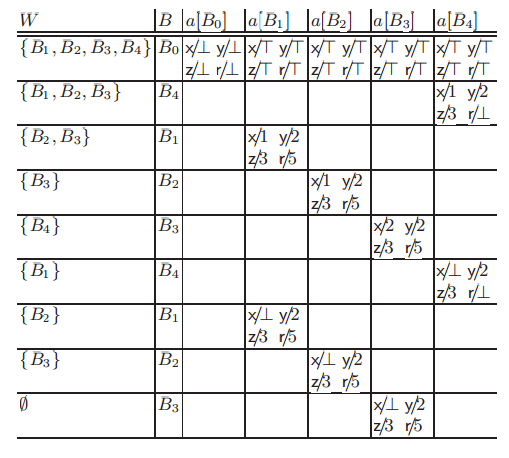
\includegraphics[scale=0.5]{classic.png}
\end{frame}

\section{New evaluation-based algorithm}
\begin{frame}{The algorithm}
\begin{itemize}
\item Uses an array of instructions $I$, a working set of program counters
$W$, and a parallel array of abstract values $a$
\end{itemize}
\end{frame}
\section{Evaluation}

\begin{frame}{References}
\bibliographystyle{plain}
{\footnotesize
\bibliography{bib}}
\end{frame}

\end{document}
